\section{Prospect study of EW-$ZZjj$ production in HL-LHC}

The High-Luminosity Large Hadron Collider (HL-LHC) project aims to increase the luminosity by a factor of 10 beyond the LHC’s design value 
to increase the potential for discoveries after 2025.
The expected luminosity will reach 3000~\ifb~with the centre-of-mass energy of 14~\tev.

As introduced in previous sections, with full run-2 data of 139~\ifb collected by ATLAS detector at the LHC, 
the EW-$ZZjj$ production is the last channel of observation for VBS processes with massive bosons 
due to its very low cross section in $ZZ$ channel.
So we expect that this channel will benefit significantly from the increased luminosity at the HL-LHC,
and can be studied in great details for this known mechanism.

In this section, a prospective study is performed for EW-$ZZjj$ production at the HL-LHC in the \llll channel~\cite{ATL-PHYS-PUB-2018-029}.
The study uses 3000~\ifb of simulated pp collision data at a centre-of-mass energy of 14~\tev~ as expected to be recorded by the ATLAS detector at the HL-LHC.
All simulated events are produced at particle-level, 
and the detector effects of leptons and jets reconstruction and identification are estimated by corrections
assuming the mean number of interactions per bunch crossing (<$\mu$>) of 200.

\subsection{The ATLAS detector at HL-LHC}

As the expectation of HL-LHC, the new Inner Tracker (ITk)~\cite{Collaboration:2285585}
 will extend the tracking acceptance capability of ATLAS detector to pseudorapidity ($|\eta|$) up to 4.0.
By including a forward muon trigger, the upgraded Muon Spectrometer~\cite{Collaboration:2285580} is also expected to provide 
muon identification capabilities to $|\eta|$ up to 4.0.
In addition, the new high granularity timing detector (HGTD)~\cite{Collaboration:2623663} designed to mitigate the pile-up (PU) effects 
is also expected to be installed in the forward region of $2.4 < |\eta| < 4.0$.
More details of expected performance of the upgraded ATLAS detector at the HL-LHC has been reported in Ref.~\cite{ATL-PHYS-PUB-2016-026}.

\subsection{Simulation}

The analysis is performed using particle-level events.
The samples are generated at $\sqrt{s} = 14~\tev$. %and with a fast simulation based on the setting for ATLAS detector at the HL-LHC.
The signal in this analysis is EW-$ZZjj$ process, while only the dominant irreducible background of QCD-$ZZjj$ is considered.
Both signal and background are generated using \textsc{Sherpa} with the NNPDF3.0NNLO PDF set.
The signal sample is modelled with two jets at Matrix Element (ME) level.
The background is generated with up to one (three) outgoing partons at NLO (LO) in pQCD.
As a quick study, other minor backgrounds such as fake backgrounds from \Zjet and top-quark processes, as well as Diboson without 4l final-state and Triboson processes are not considered in this analysis.
Furthermore, for hard scattering events, the pile-up collisions are set with a mean value of 200 interactions per bunch crossing.
Signal and background yields are then scaled to an integrated luminosity of 3000~\ifb~as expected at the HL-LHC.

\subsection{Event selection}

The analysis selection follows closely to the one in ATLAS run-2 analysis as described in section~\ref{sec:vbszz_selection}.
Here are some changes according to the expectation of the HL-LHC scenario for ATLAS detector:
\begin{itemize}
	\item Extend the lepton (both electron and muon) identification to $|\eta| <$ 4.0
	\item Pile-up (PU) jet suppression is applied with a PU rejection factor of 50 for all PU jets in the region of $|\eta| <$ 3.8, based on the expected ATLAS detector performance at the HL-LHC.
	\item The jets are required to have $\pT >$ 30 (70)~\gev~in the $|\eta| <$ 3.8 ($3.8 < |\eta| < 4.5)$ region.
	\item For two selected jets, tighten the $\mjj$ requirement to be $\mjj > 600$~\gev, and require $\Delta \eta_{jj} >$ 2.
\end{itemize}
In addition, a fiducial volume, used to study the expected precision of the cross-section measurements,
 is defined at particle-level with the same kinematic requirements listed above.

Table~\ref{tab:event_yield} summarized the number of selected signal and background events normalized to 3000~\ifb.
In addition to the \textit{baseline} selection listed above, to compare the different detector scenarios at the HL-LHC, two alternative selections are also studied:
\begin{enumerate}
	\item Reduce the lepton $\eta$ region to 2.7, to understand the effect due to forward lepton reconstruction and identification with the upgraded ATLAS detector.
	\item Only apply the PU jet suppression with region $|\eta| < 2.4$, to measure the improvement of \textit{baseline} by extending the rejection range of PU jets at the HL-LHC with the installation of HGTD.
\end{enumerate}
\begin{table}[htbp]
  \small
  \centering
  \begin{tabular}{|c|c|c|c|}
    \hline
    Selection & $N_{\mathrm{EW-ZZjj}}$ & $N_{\mathrm{QCD-ZZjj}}$ & $N_{\mathrm{EW-ZZjj}}$ / $\sqrt{N_{\mathrm{QCD-ZZjj}}}$ \\
    \hline
    Baseline                                 & 432 $\pm$ 21 & 1402 $\pm$ 37   & 11.54 $\pm$ 0.58 \\
    \hline
    Leptons with $|\eta|<$ 2.7               & 373 $\pm$ 19 & 1058 $\pm$ 33   & 11.46 $\pm$ 0.62 \\
    \hline
    PU jet suppression only in $|\eta|<$ 2.4 & 536 $\pm$ 23 & 15470 $\pm$ 120 &  4.31 $\pm$ 0.19  \\
    \hline
  \end{tabular}
  \caption{
    Comparison of event yields for signal ($N_{\mathrm{EW-ZZjj}}$) and background ($N_{\mathrm{QCD-ZZjj}}$) processes, 
    and expected significance of EW-$ZZjj$ processes,
    normalized to 3000~\ifb{} data at 14~\TeV{},
    with baseline and alternative selections.
    Uncertainties in the table refer to expected data statistical uncertainty at 14~\TeV{} with 3000~\ifb{}.
  }
  \label{tab:event_yield}
\end{table}
From this table, one can see the extended track coverage increases the \lllljj events by 15 to 30\%, via improving the lepton efficiency.
But the significance of searching for EW-$ZZjj$ process does not improve so much due to the large increment of background events.

Figure~\ref{fig:kine} shows the kinematic distributions of di-jet invariant mass (\mjj), the $ZZ$ invariant mass (\mzz) and 
the $\phi$ separation of two Z bosons ($|\Delta\phi(ZZ)|$) as well as the centrality of the ZZ system.
The ZZ centrality is defined as:
\begin{equation}
  ZZ~\text{centrality} = \frac{|y_{ZZ} - (y_{j1} + y_{j2})/2|}{|y_{j1} - y_{j2}|}
\end{equation}
To measure the event yield, the top panel shows the stack distribution for EW- and QCD-$ZZjj$ processes,
while bottom panel is the ratio between two processes.
\begin{figure}[!htbp]
\centering
\subfloat[]{
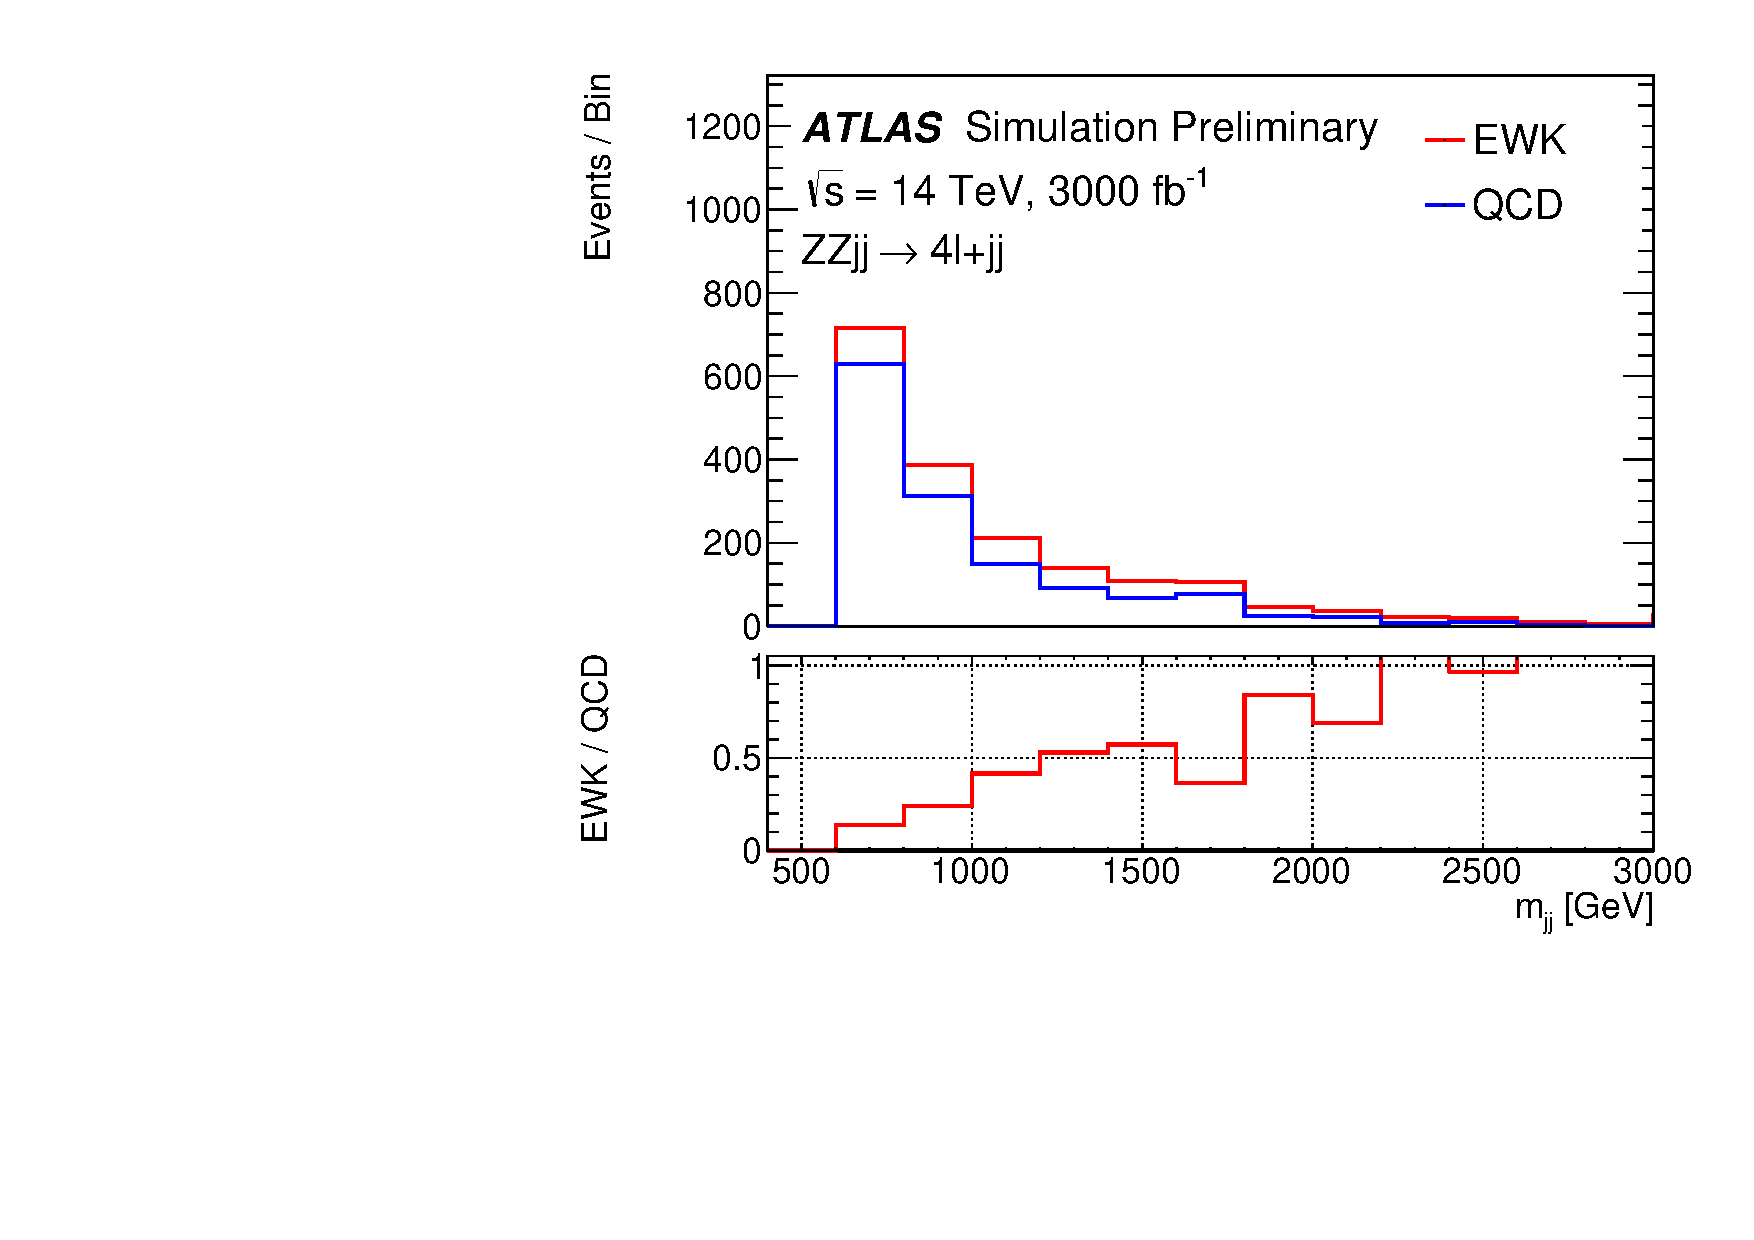
\includegraphics[width=0.42\textwidth]{figures/VBSZZ/hllhc/TagJJM_final_noshape_0_ratio.pdf}
}
\subfloat[]{
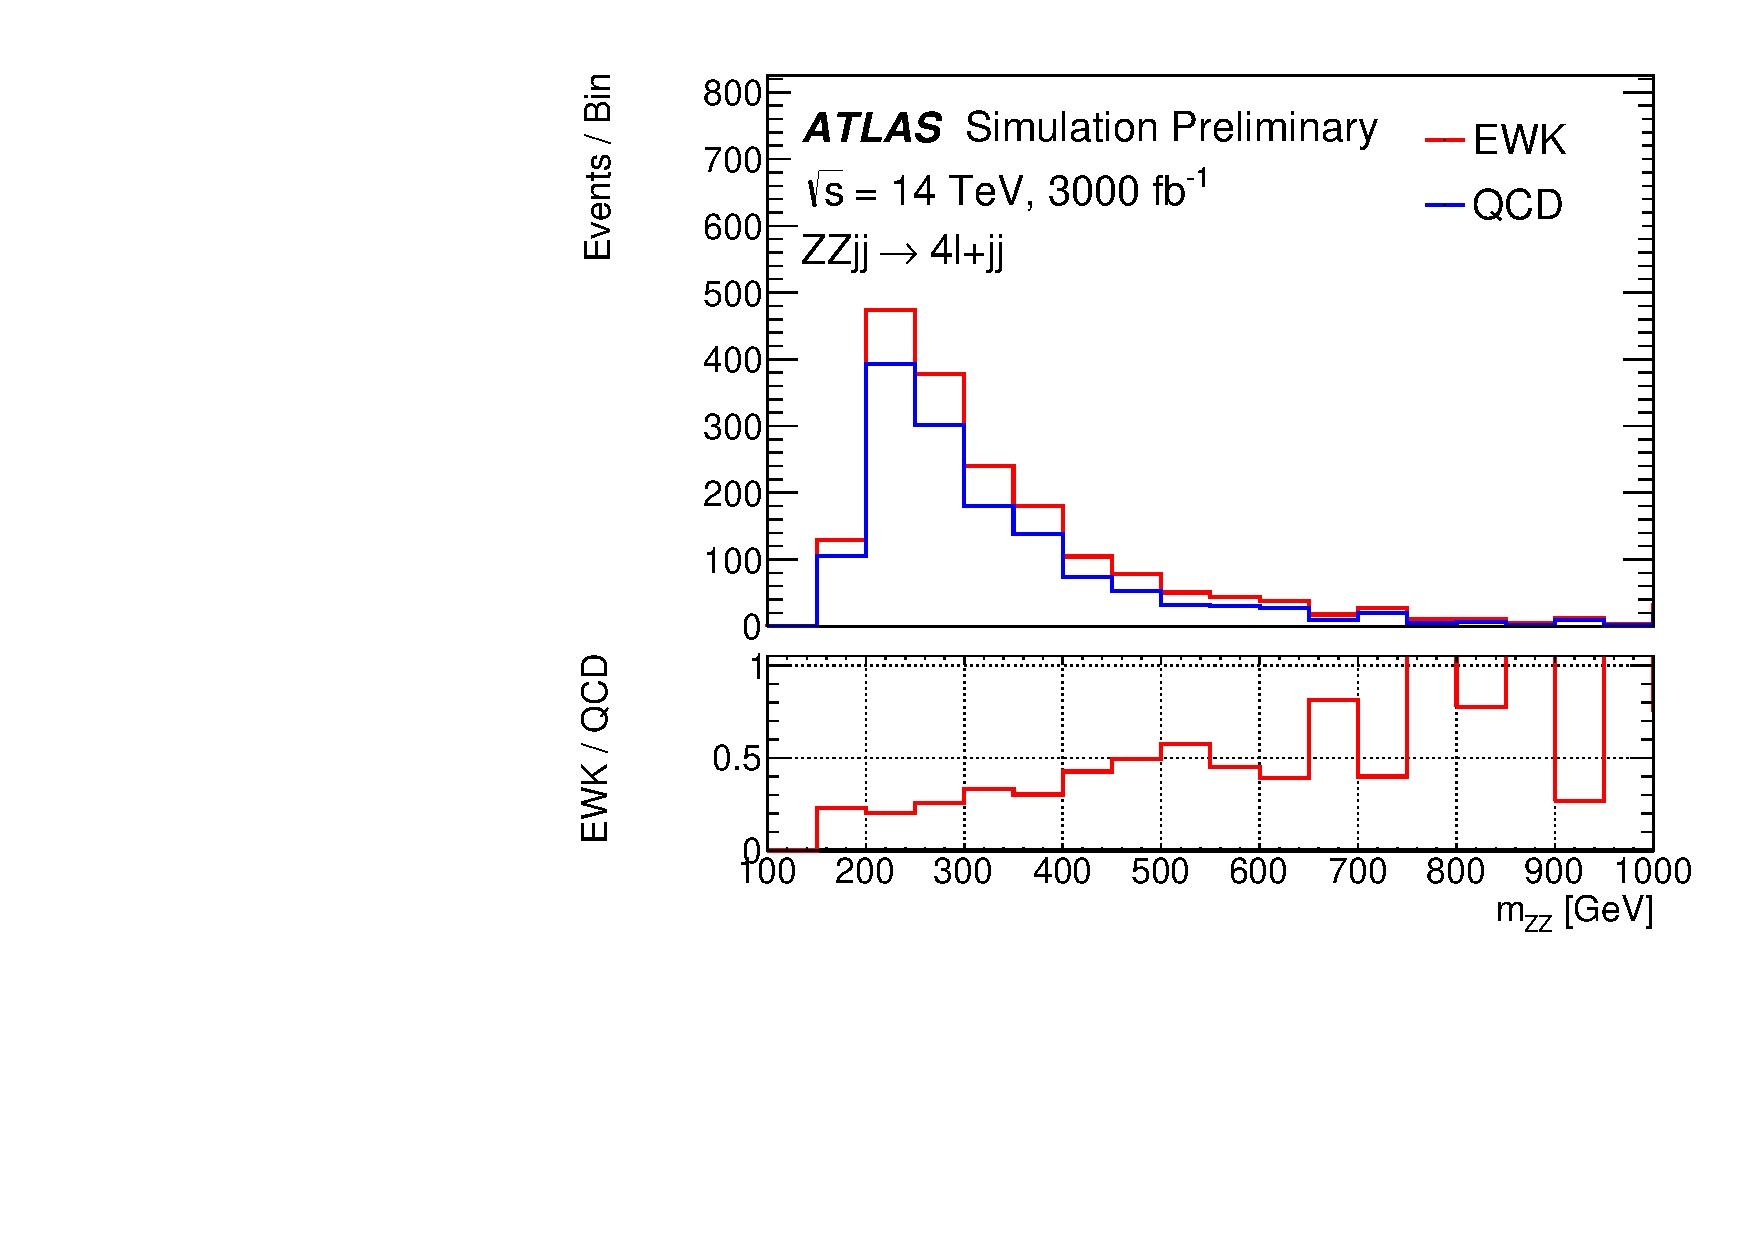
\includegraphics[width=0.42\textwidth]{figures/VBSZZ/hllhc/MVV_noshape_0_ratio.pdf}
}
\\
\subfloat[]{
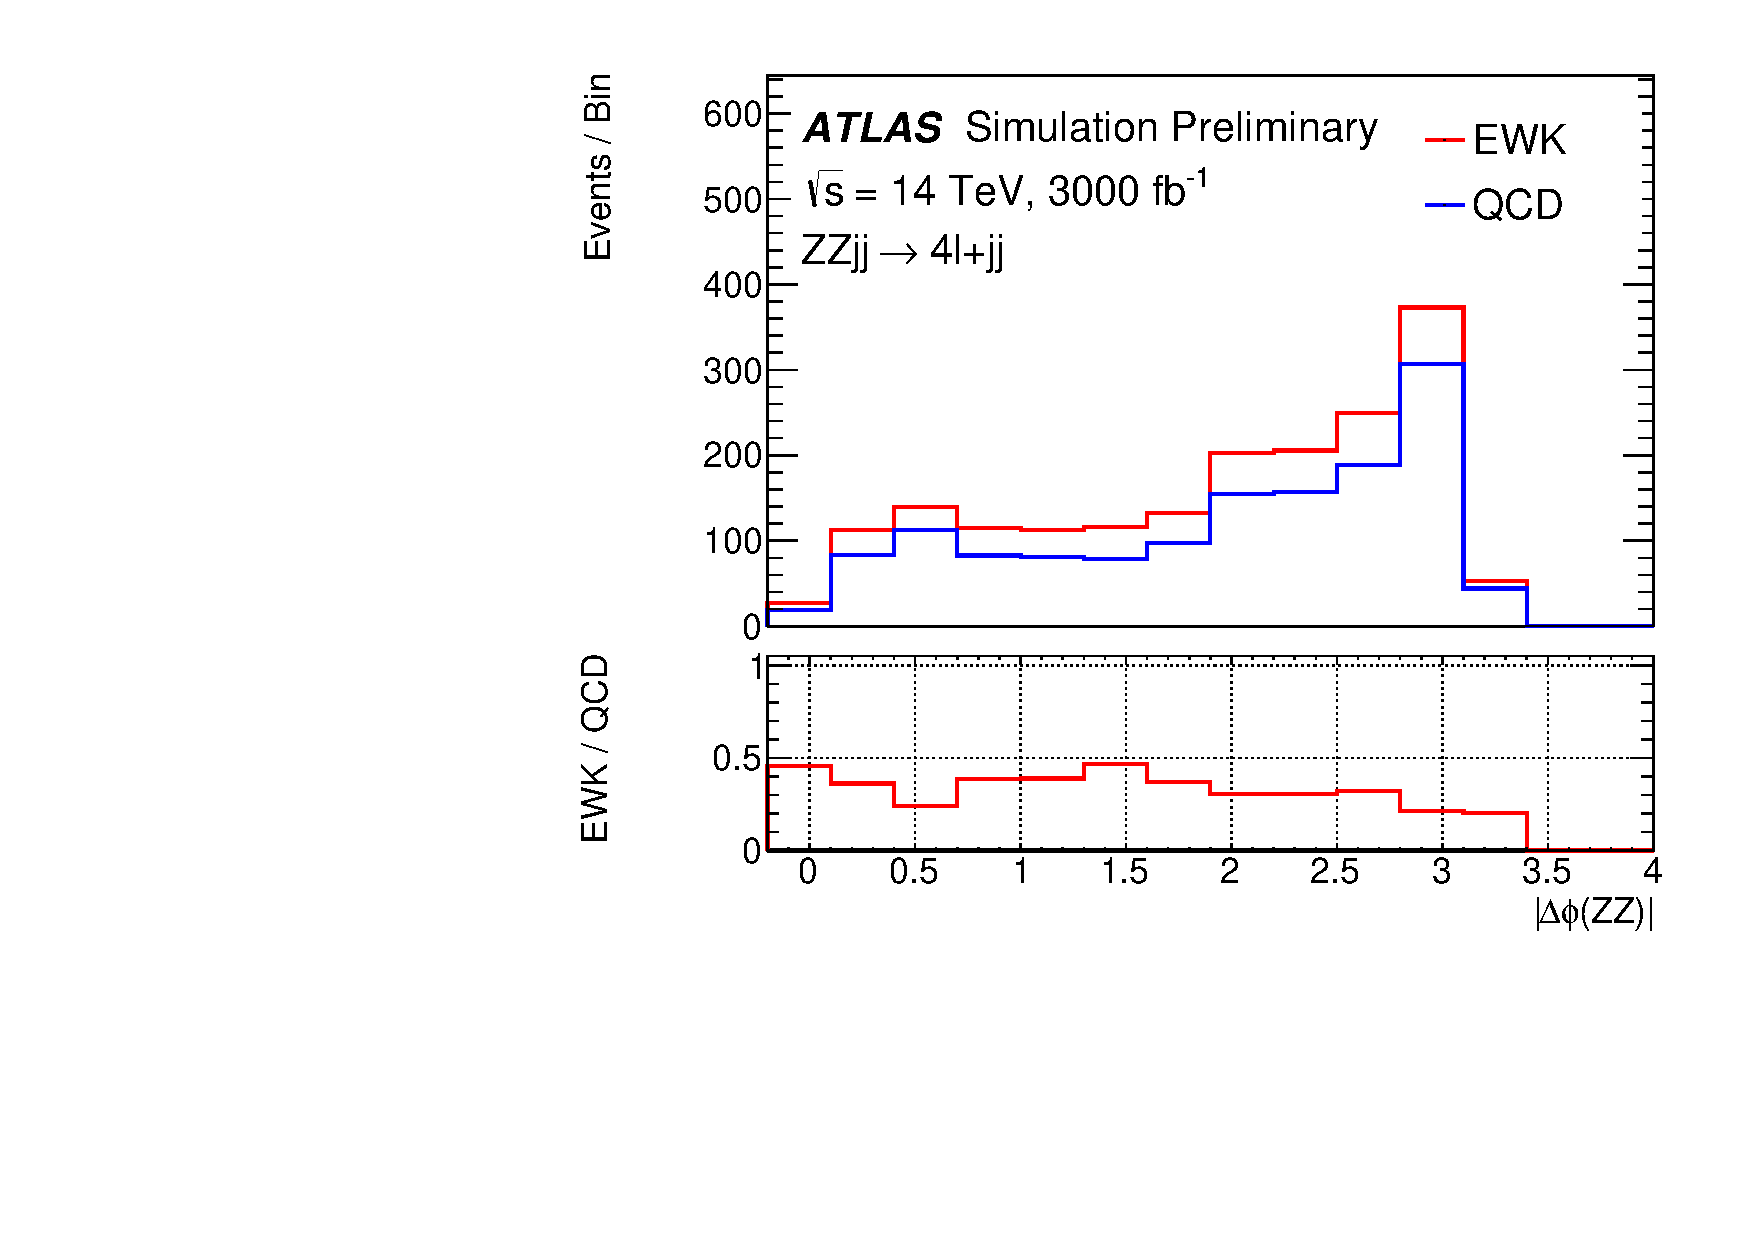
\includegraphics[width=0.42\textwidth]{figures/VBSZZ/hllhc/dPhiZZ_noshape_0_ratio.pdf}
}
\subfloat[]{
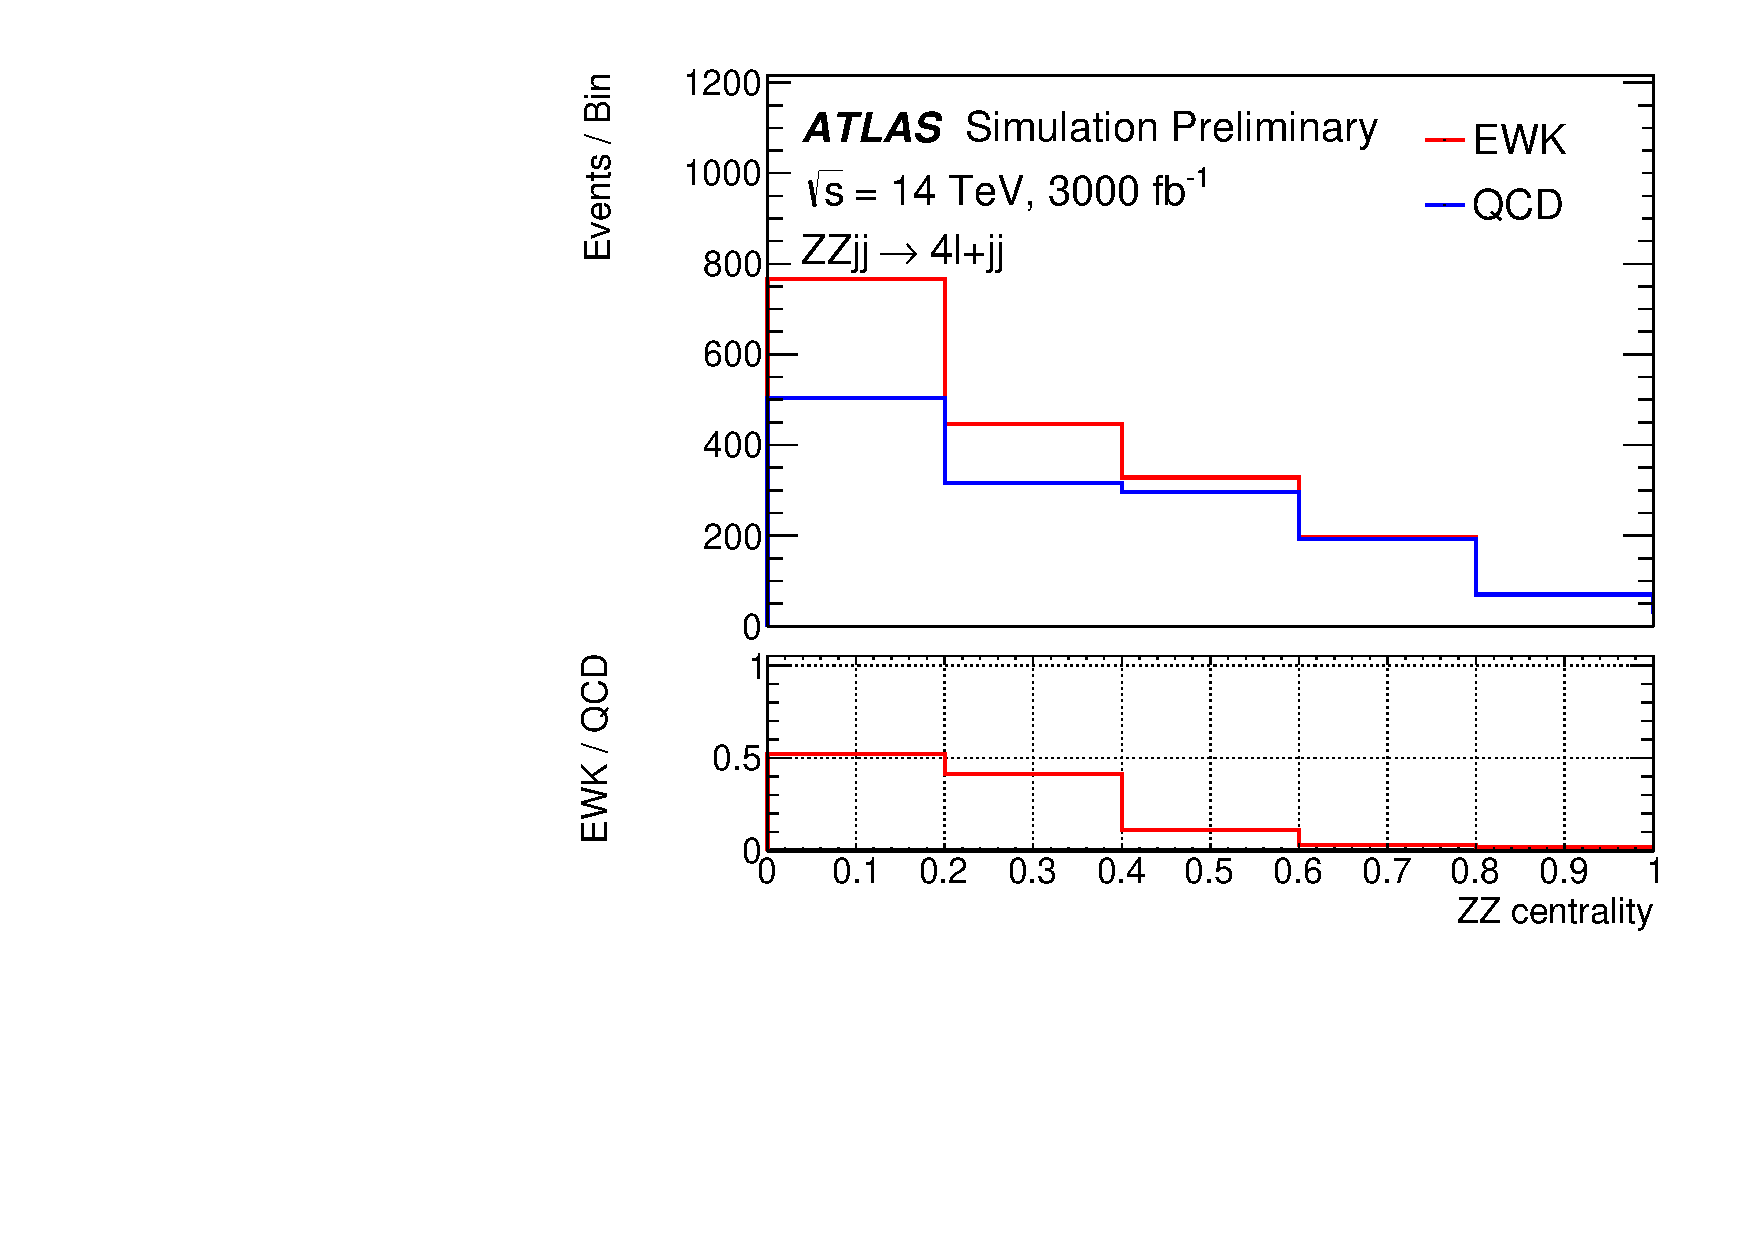
\includegraphics[width=0.42\textwidth]{figures/VBSZZ/hllhc/ZZCen_noshape_0_ratio.pdf}
}
\caption{
Detector-level distributions of EW- and QCD-$ZZjj$ processes with selected events in defined phase space at 14~\tev~of 
(a) \mjj,
(b) \mzz,
(c) $|\Delta\phi(ZZ)|$,
(d) ZZ centrality,
normalized to 3000~\ifb{}.
}
\label{fig:kine}
\end{figure}


\subsection{Systematics}

According to studies in section~\ref{sec:systematics}, the dominant systematic in \llll channel is from theoretical systematic for QCD-$ZZjj$ background process.
Different sizes of systematics have been studied, at a factor of 5, 10 and 30\% on background modelling.
The 5\% uncertainty is an optimal estimation when there is enough data events from QCD-enriched control region at the HL-LHC that can be used to constrain the theoretical normalization on QCD-$ZZjj$ process.
The 30\% one is a conservative estimation, in which the uncertainties are directly calculated from different PDF sets and QCD renormalization and factorization scales, following recommendation from the PDF4LHC mentioned in section~\ref{sec:systematics}.

For experimental sources, the jet systematics have been checked following the setting provided by the HL-LHC in Ref.\cite{ATL-PHYS-PUB-2016-026},
and the uncertainties are within 5\% level, which is smaller than run-2 measurement at 10\%.
Figure~\ref{fig:jet_uncer} depicts the up and down variations for jet uncertainty provided by the HL-LHC performance tool as function of dijet invariant mass ($\mjj$).
\begin{figure}
  \centering
  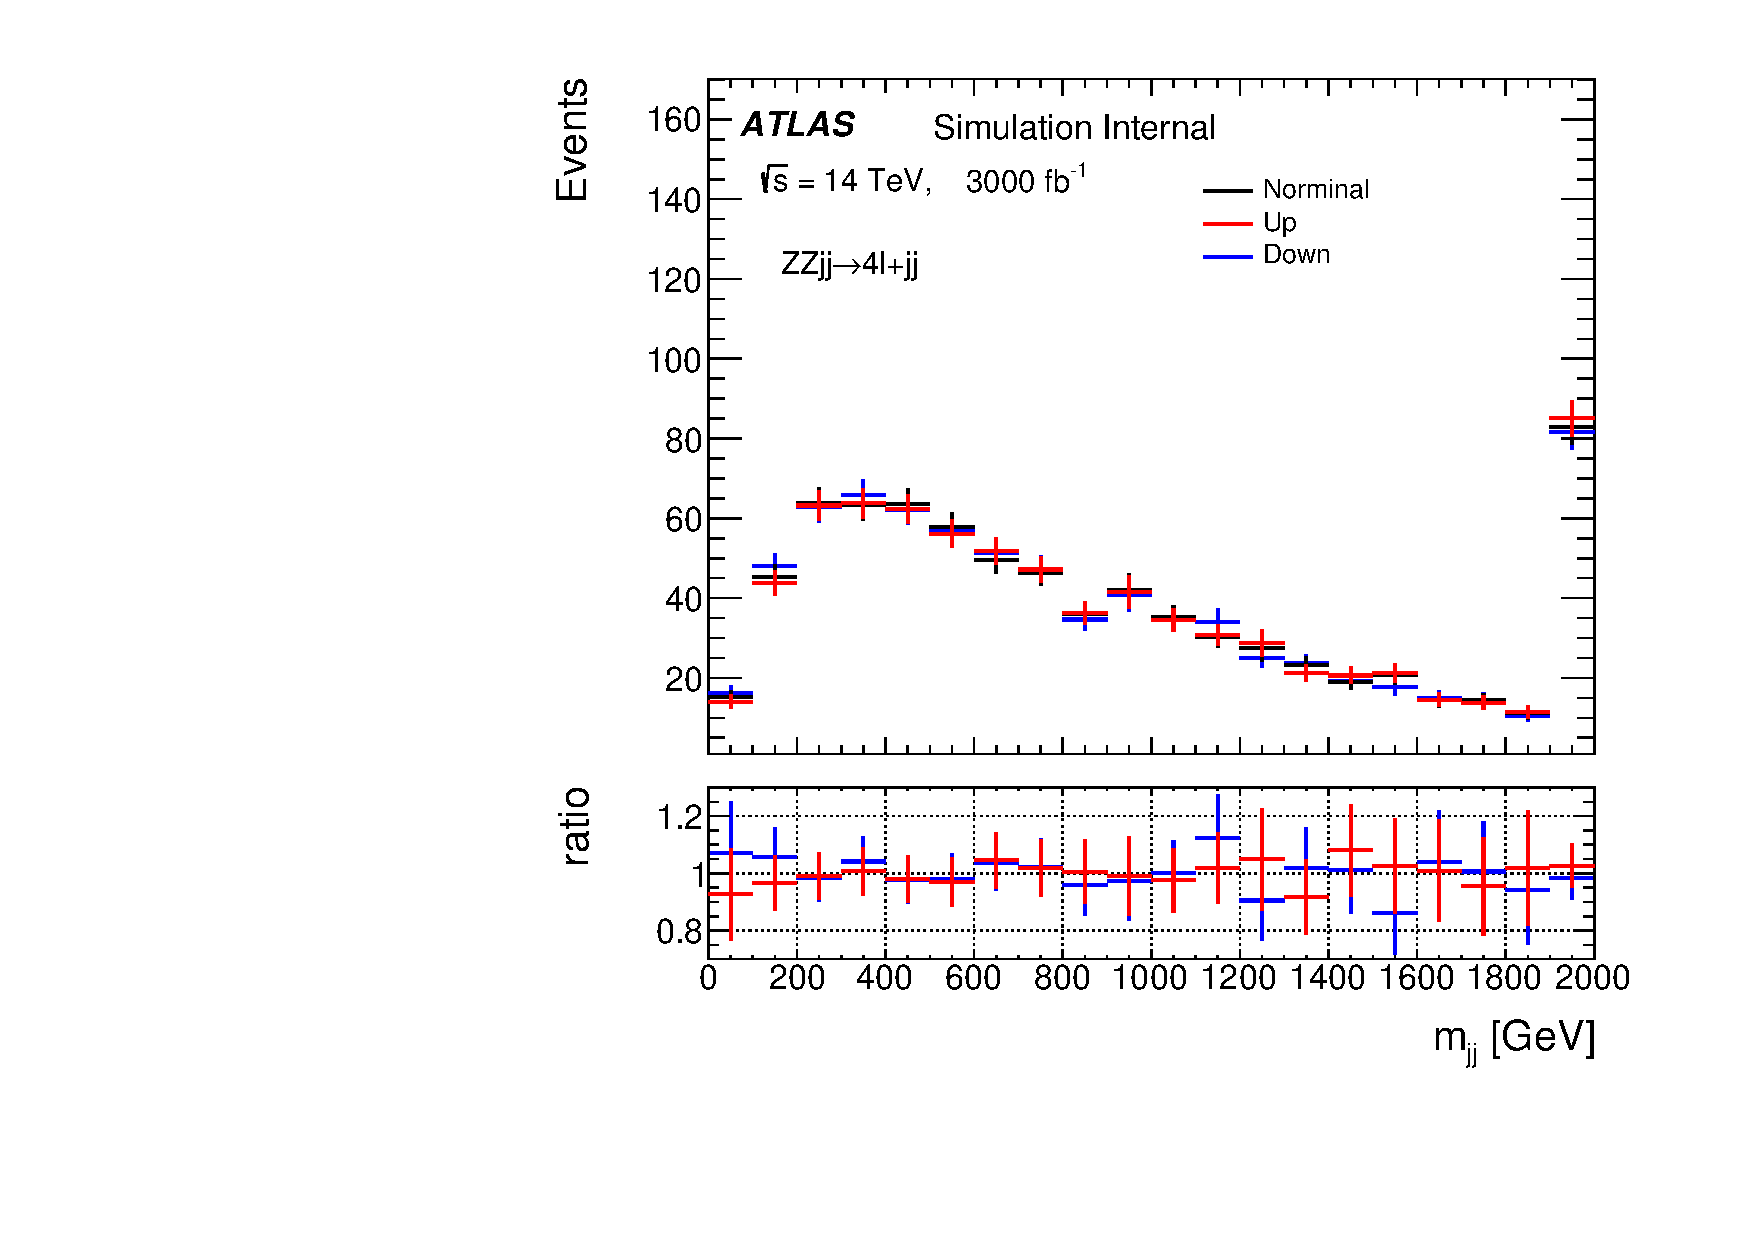
\includegraphics[width=0.42\textwidth]{figures/VBSZZ/hllhc/Uncer_baseline_TagJJM_ewk_linear.pdf}
  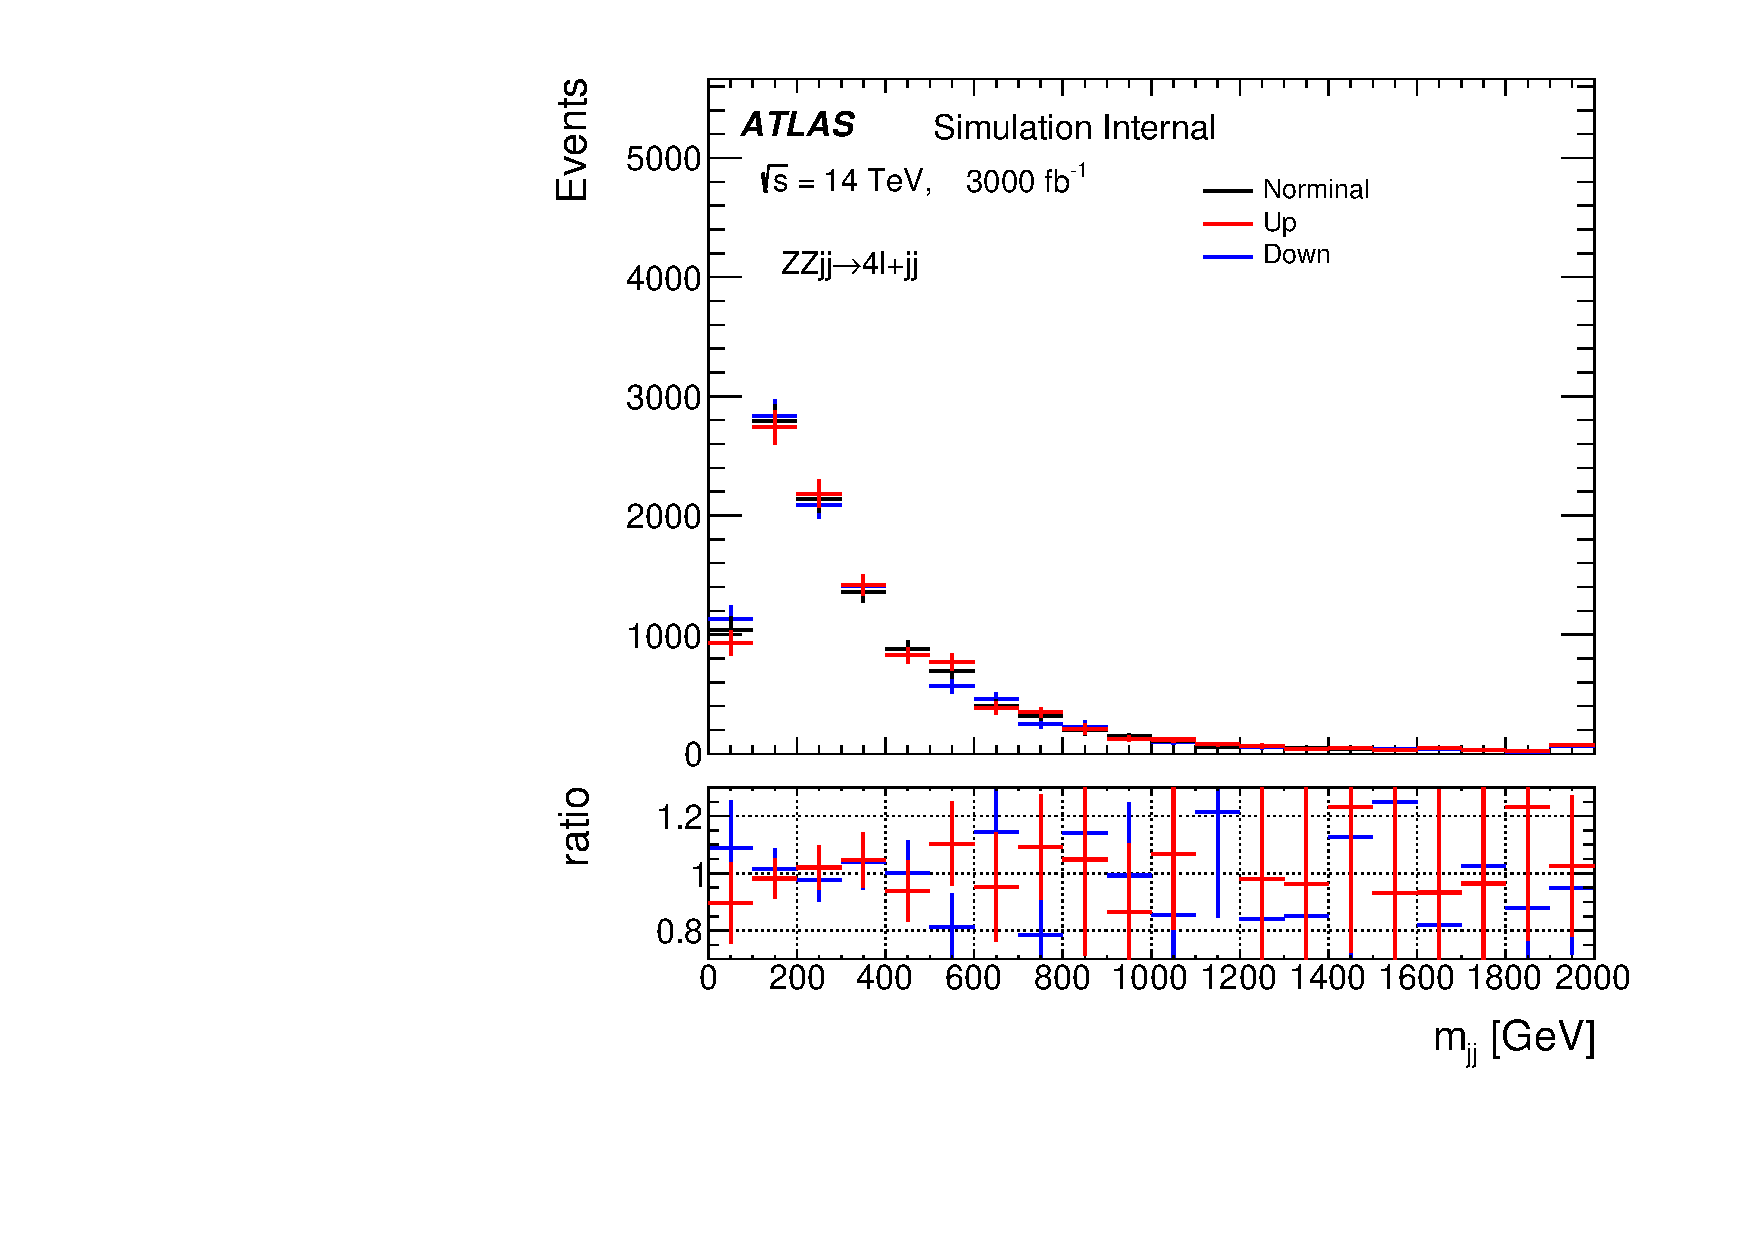
\includegraphics[width=0.42\textwidth]{figures/VBSZZ/hllhc/Uncer_baseline_TagJJM_qcd_linear.pdf}
  \caption{Jet variations on $\mjj$ distribution for EW-$ZZjj$ (left) and QCD-$ZZjj$ (right) processes
           with luminosity of 3000~\ifb at 14~\tev.
	   \textit{Upgrade Performance Function} is used to extract the uncertainties with \textit{baseline} setting.}
  \label{fig:jet_uncer}
\end{figure}
Therefore, a conservative 5\% uncertainty is used as experimental uncertainty.

Since the final result relies greatly on the uncertainties, especially the theoretical uncertainties on QCD-$ZZjj$ production.
So results with different uncertainty conditions are shown as below:
\begin{itemize}
	\item The case with statistical uncertainty of simulated samples only.
	\item The case with statistical and experimental uncertainties (5\%)
	\item The case with statistical, experimental and additional theoretical uncertainties at 5\%, 10\% and 30\% levels respectively.
\end{itemize}
Three different sources of uncertainties are treated as uncorrelated and summed up quadratically.

\subsection{Results}

In this analysis, instead of a statistical fit, the expected significance of EW-$ZZjj$ production is calculated as:
\begin{equation}
  \text{Significance} = \frac{S}{\sqrt{\sigma(B)_{stat.}^2 + \sigma(B)_{syst.}^2}},
\end{equation}
where $S$ presents the number of selected signal events,
and $\sigma(B)_{stat.}$ and $\sigma(B)_{syst.}$ denote the statistical and systematic (exp. + theo.) uncertainties from background processes.
The statistical uncertainty is computed from expected data yield with an integrated luminosity of 3000~\ifb.

Based on baseline selection of $\mjj > 600~\gev$, an additional scan over different \mjj cuts is also performed with a step of 50~\gev~
under different systematic conditions, as shown in figure~\ref{fig:mjj_scan}.
\begin{figure}[!htbp]
\centering
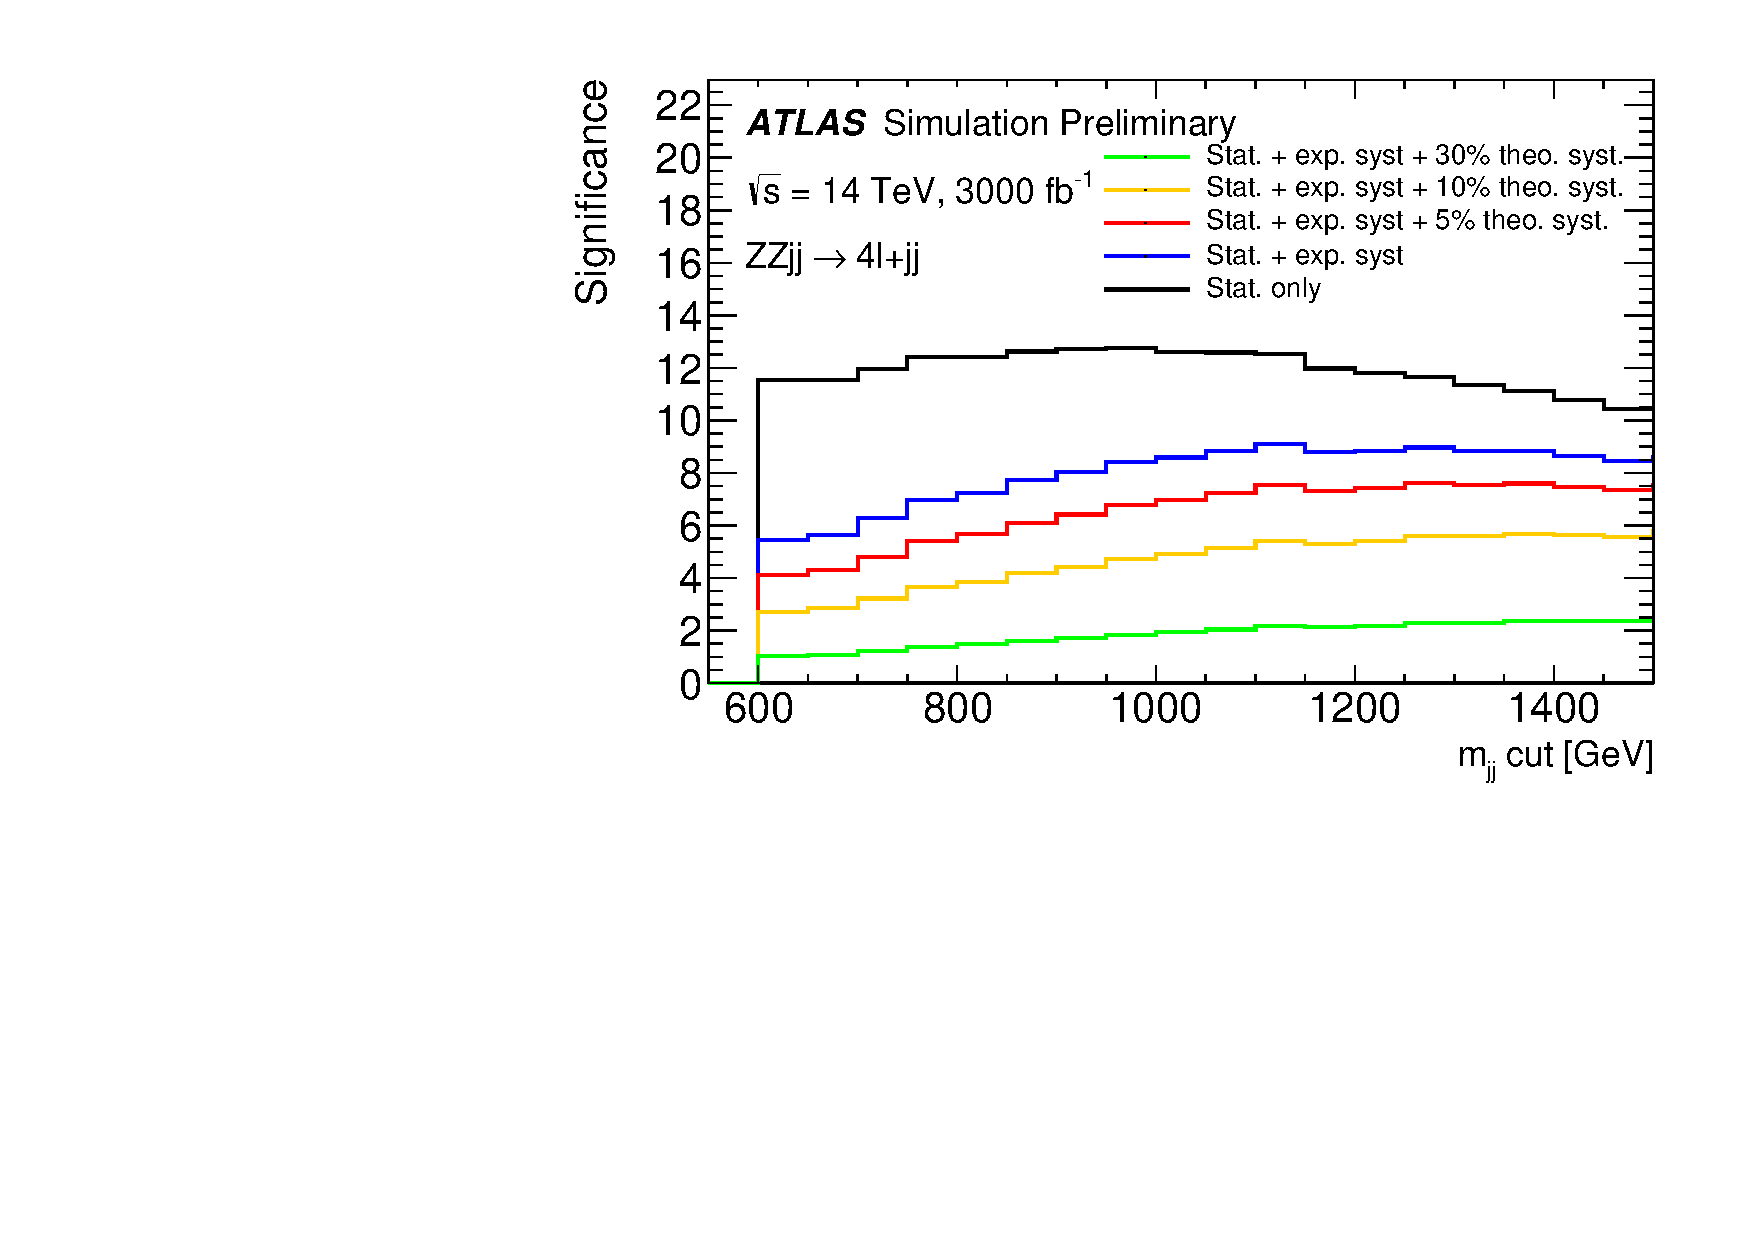
\includegraphics[width=0.48\textwidth]{figures/VBSZZ/hllhc/significance_noshape_0_noratio.pdf}
\caption{
The expected significance of EW-$ZZjj$ processes as a function of different \mjj cut with 3000~\ifb,
under conditions of different sizes of theoretical uncertainties on the QCD-$ZZjj$ background modelling.
The statistical uncertainty is estimated from expected data yield at 14~\tev~ with 3000~\ifb.
Different uncertainties are summed up quadratically.
}
\label{fig:mjj_scan}
\end{figure}

In addition, the expected differential cross section of EW-$ZZjj$ process is measured in the defined phase space at 14~\tev,
as a function of \mzz and \mjj, shown in figure~\ref{fig:xs_mjj_mzz}.
\begin{figure}[!htbp]
\centering
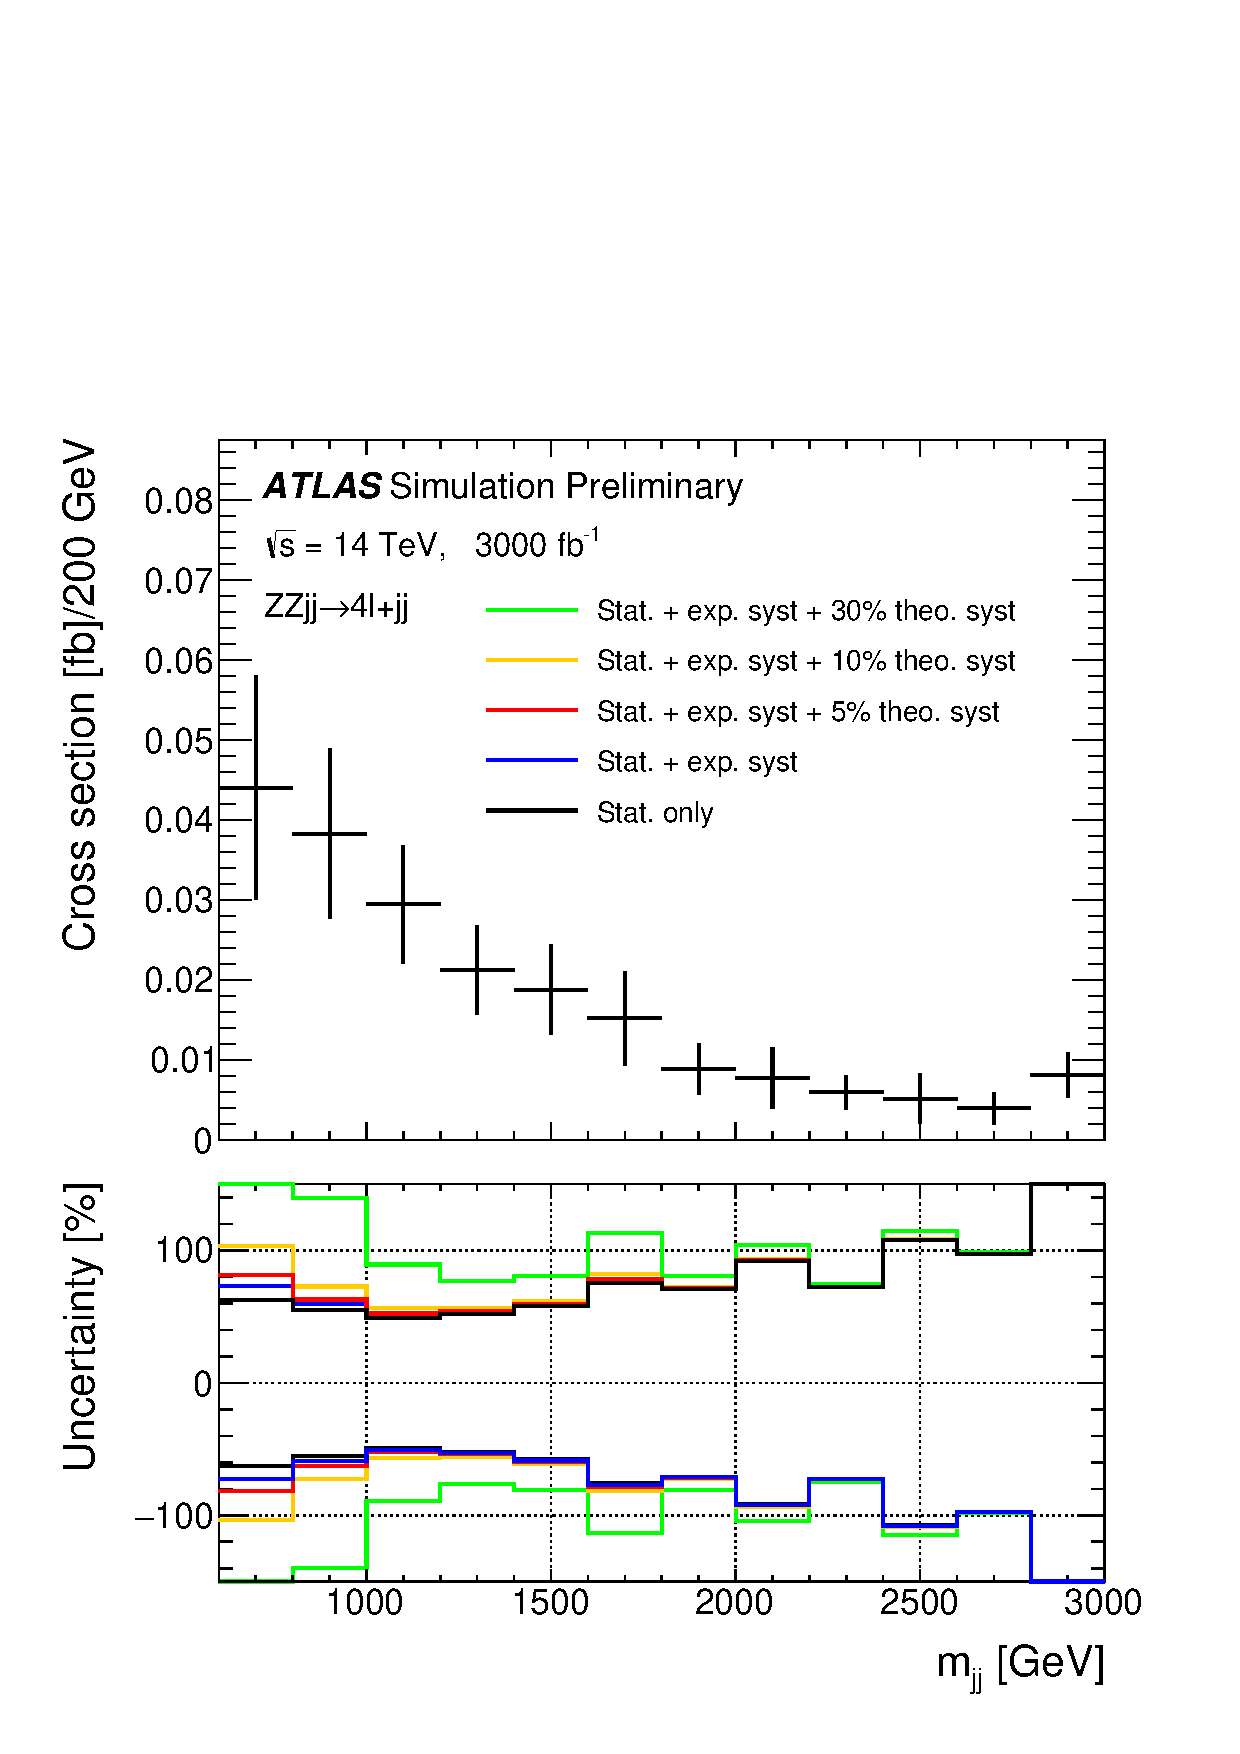
\includegraphics[width=0.48\textwidth]{figures/VBSZZ/hllhc/TagJJM_final_all_linear.pdf}
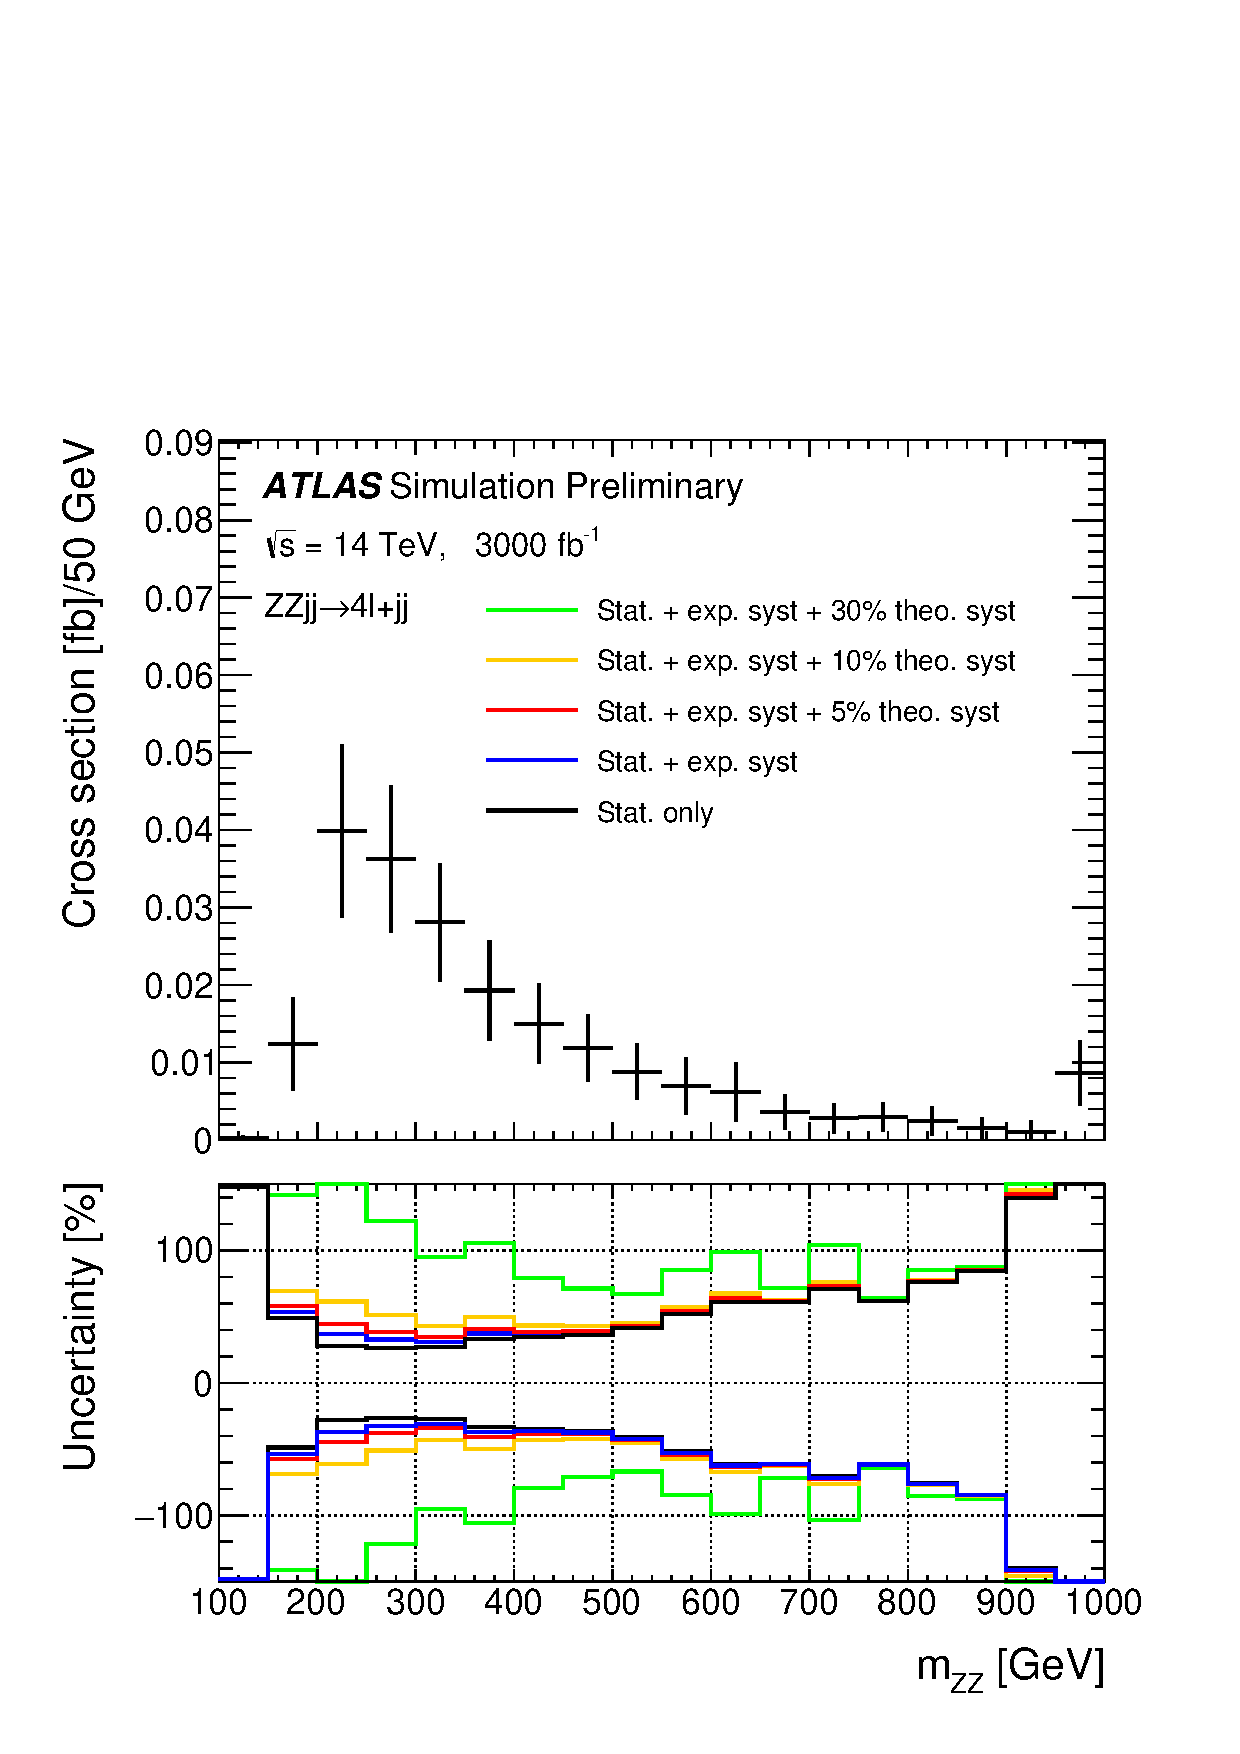
\includegraphics[width=0.48\textwidth]{figures/VBSZZ/hllhc/MZZ_all_linear.pdf}
\caption{
The projected differential cross-sections at 14~\tev~ for the EW-$ZZjj$ processes as a function of \mjj (left) and \mzz (right).
The top panel shows measurement with statistical only case,
where statistical uncertainty is estimated from expected data yield at 14~\tev~ with 3000~\ifb.
The bottom panel shows impact of different sizes of systematic uncertainties.
}
\label{fig:xs_mjj_mzz}
\end{figure}
The expected differential cross sections are calculated as:
\begin{equation}
\begin{split}
  \sigma = \frac{N_{pseudo-data} - N_{QCD-ZZjj}}{L*C_{EW-ZZjj}}\\
  C_{EW-ZZjj} = \frac{N_{EW-ZZjj}^{det.}}{N_{EW-ZZjj}^{part.}}
\end{split}
\end{equation}
where $N_{pseudo-data}$ denotes the expected number of data events with 3000~\ifb~ luminosity at 14~\tev,
and $N_{QCD-ZZjj}$ and $N_{EW-ZZjj}$ are the number of predicted events of QCD-$ZZjj$ and EW-$ZZjj$ processes in particle-level.
The $C_{EW-ZZjj}$ factor represents the detector efficiency for EW-$ZZjj$ processes introduced in section~\ref{sec:cf}.
The interference between EW- and QCD- $ZZjj$ processes is ignored due to its minor contribution.

The value of expected integrated cross section as well as its uncertainty under different systematic conditions are shown in table~\ref{tab:xsec}
with 3000~\ifb luminosity at 14~\tev.
The statistical uncertainty is at 10\% level when with such large luminosity.
The result is dominated by systematics and can reach 100\% level when theoretical modelling uncertainty is 30\% for QCD-$ZZjj$ processes.
\begin{table}[htbp]
  \footnotesize
  \centering
  \begin{tabular}{c|c|c|c|c|c|c}
    \hline
     & Cross section [fb] & Stat. only & Plus exp. & Plus $5\%$ theo. & Plus $10\%$ theo. & Plus $30\%$ theo. \\
    \hline
    EW-$ZZjj$ & 0.21 & $\pm0.02$ & $\pm0.04$ & $\pm0.05$ & $\pm 0.08$ & $\pm 0.21$ \\
    \hline
  \end{tabular}
  \caption{
  Summary of expected cross-section measured with different theoretical uncertainties.
  The statistical uncertainty is computed from expected data yield with 3000~\ifb~ at 14~\tev.
  Different uncertainties are treated as uncorrelated and summed quadratically.
  }
  \label{tab:xsec}
\end{table}

